\section{Optimization}
To maximize the cumulative discounted profit in a framework of NaaA,
it is important to balance the two contradicting criteria: revenue $r_{it}$ and cost $c_{it}$.

%TODO: Negative result. State what is the problem.
%\begin{thm}\label{thm:optimal-bidding-simple}
%	The Nash equivalent of the game $(\rho_{ijt})$ is $0$.
%\end{thm}

To achieve that, we use the mechanism design.
We introduce mechanism design because, unlike several existing studies \citep{sukhbaatar2016learning}, NaaA assumes that all agents are not cooperative but selfish.
%(TODO: Bad writing.)
If we naively optimize the optimization problem of NaaA, then we obtain the trivial solution that the internal rewards will converge to 0, and that all the units become NOOP.
Therefore, the multi-agent system should select the action with no information. It is equivalent to taking an action randomly.
For that reason, the external reward $R_t^{\mathrm ex}$ shrinks markedly.

\subsection{Envy-free Auction}
To achieve Pareto optimality, we borrow the idea from the digital goods auction.
The auction theory belongs to mechanism design. It is intended to unveil the true price of goods.
Digital goods auction is one mechanism from auction theory.
It is target to copyable goods without cost, such as digital books and music.

Although several variations of digital goods auctions exist,
we use an envy-free auction \citep{guruswami2005profit} because it requires a simple assumption: the same goods have one price simultaneously.
In NaaA, it can be represented as the following assumption:
\begin{enumerate}
\renewcommand{\labelenumi}{N\arabic{enumi}:}
\setcounter{enumi}{4}
\item (Law of one price)
	If $\rho_{j_1,i,t}, \rho_{j_2,i,t} > 0$, then $\rho_{j_1,i,t} = \rho_{j_2,i,t}$.
\end{enumerate}
Therefore, $\unit$ has an intrinsic price at the same timing $t$.
We denote the price as $q_{it}$.

%TODO: Describe for allocation

We present the envy-free auction process at the left of Figure \ref{fig:double}.
It shows the negotiation process between one unit in sending activation and a group of units that buy the activation.
The negotiation performed per time step in RL.
We name the unit in sending activation as a seller, and units in buying activation as buyers.
First, the buyer bids the unit in bidding price $b_{jit}$ (\textbf{1}).
Next, the seller decides the optimal price $\opt{q}_{it}$, and performs allocation (\textbf{2}).
Payment occurs if $b_{ijt}$ exceeds $q_{jt}$.
In this case, $\rho_{jit} = H(b_{jit} - q_{it}) q_{it}$ holds where $H(\cdot)$ is a step function.
Besides, we define $g_{jit} = H(b_{jit} - q_{it})$ and name it {\em allocation}.
After allocation, the buyers perform payment as $\rho_{jit} = g_{jit} \opt{q}_{it}$ (\textbf{3}).
Eventually, seller earns 
The seller only sends activation $x_i$ to the allocated buyers (\textbf{4}).
A buyer which cannot receive the activation approximates $x_i$ with $\Expect{\pi}{x_i}$.

In the following, we discuss revenue, cost, and value functions based on Eq:(\ref{eq:V}).



%========================================
% 収益
%========================================

\textbf{Revenue}:
The revenue of a unit is given as
\begin{flalign}
	r_{it}  &= \sum_{j \in N^\mathrm{out}_i} g_{jit} q_{it} + R^\mathrm{ex}_i \\
		&= q_i d_{it} + R^\mathrm{ex}_i,
\end{flalign}
where $d_{it} = \sum_{j \in N^\mathrm{out}_i} g_{jit}$ is a count of units for which the bidding price for $q_{it}$ is greater than or equal to $q_{it}$, designated as demand.
$q_{it}$ maximizing the equation is designated as the optimal price. It is denoted as $ \opt{q}_{it} $.
Because the second term in the equation is independent of $q_t$, the optimal price $\opt{q}_{it}$ is given as
\begin{flalign}
	\opt{q}_{it}  = \argmax_{q \in [0, \infty)} q d_{it}(q).
\end{flalign}
We present the curve of $q_{it}$ on the right side of Figure \ref{fig:double}.

%========================================
% コスト
%========================================
\textbf{Cost}:
The cost is an internal reward that the unit should pay to other units.
It is represented as shown below.
\begin{flalign}
	c_{it} = \sum_{j \in N^\mathrm{in} } g(b_{ijt}, q_j) q_j
\end{flalign}
Although $c_{it}$ itself is minimized when $b_{ijt} = 0$,
this represents a tradeoff with the following value function.

\textbf{Value Function}:
%Value of the value function $V(s_{i,t+1})$ depends on $s_{i,t+1}$.
%As we already defined, the internal environment of $v_i$ is a set of connected units,
%and the output of units affect to evaluation from the units, namely, weight of edges.
%As the learning rule of a typical artificial neural network obeys to law of Hebb, 
%the reward becomes lower because weight of unit which do not contribute
%the accuracy of output becomes lower.
Activation $x_i$ depends on input from the units in $N_i^{\mathrm in}$. It affects the bidding price from units in $N_i^{\mathrm out}$.
If we minimize $b_{ijt}$ and let $b_{ijt} = 0$, then the purchase of activation fails, and the reward the unit can obtain from the units to which 
the unit connects becomes lower in the future.

Then, we designate the allocation as $\vect{g}_{it} = (g_{i1t}, \dots, g_{iNt})^\T$, 
and consider effects for value functions in the cases when a unit succeeds in purchasing $v_j$ or not.
The value function can be written as the equation using a state-value function $Q(s_{i,t+1}, \vect{g}_{i,t+1})$.
\begin{flalign}
	V_i^{\pi_i}(s_{it}) 
	&= Q_i^{\pi_i}(s_{it}, \vect{g}_{it}) \notag \\
	&= \sum_{j \in \followees} g_{ijt} (Q_i^{\pi_i} (s_{it}, \vect{e}_j) - Q_i^{\pi_i}(s_{it}, \vect{0})) + Q_i^{\pi_i}(s_{it}, \vect{0}) \notag \\
	&= \sum_{j \in \followees} g_{ijt} o_{ijt} + Q_i^{\pi_i}(s_{it}, \vect{0}) \notag \\
	&= \vect{g}_{it}^\T \vect{o}_{it} + Q_i^{\pi_i}(s_{it}, \vect{0})
\end{flalign}

We designate $o_{ijt} = Q_i^{\pi_i} (s_{it}, \vect{e}_j) - Q_i^{\pi_i}(s_{it}, \vect{0})$ as the {\em counterfactual return}, 
which is equivalent to the cumulative discount value of counterfactual reward \citep{agogino2006quicr}.
That is, the cost the unit will pay is $\opt{q}_{it}$ in success of purchasing data, and $o_{it}$ otherwise.

\begin{figure*}[t]
\centering
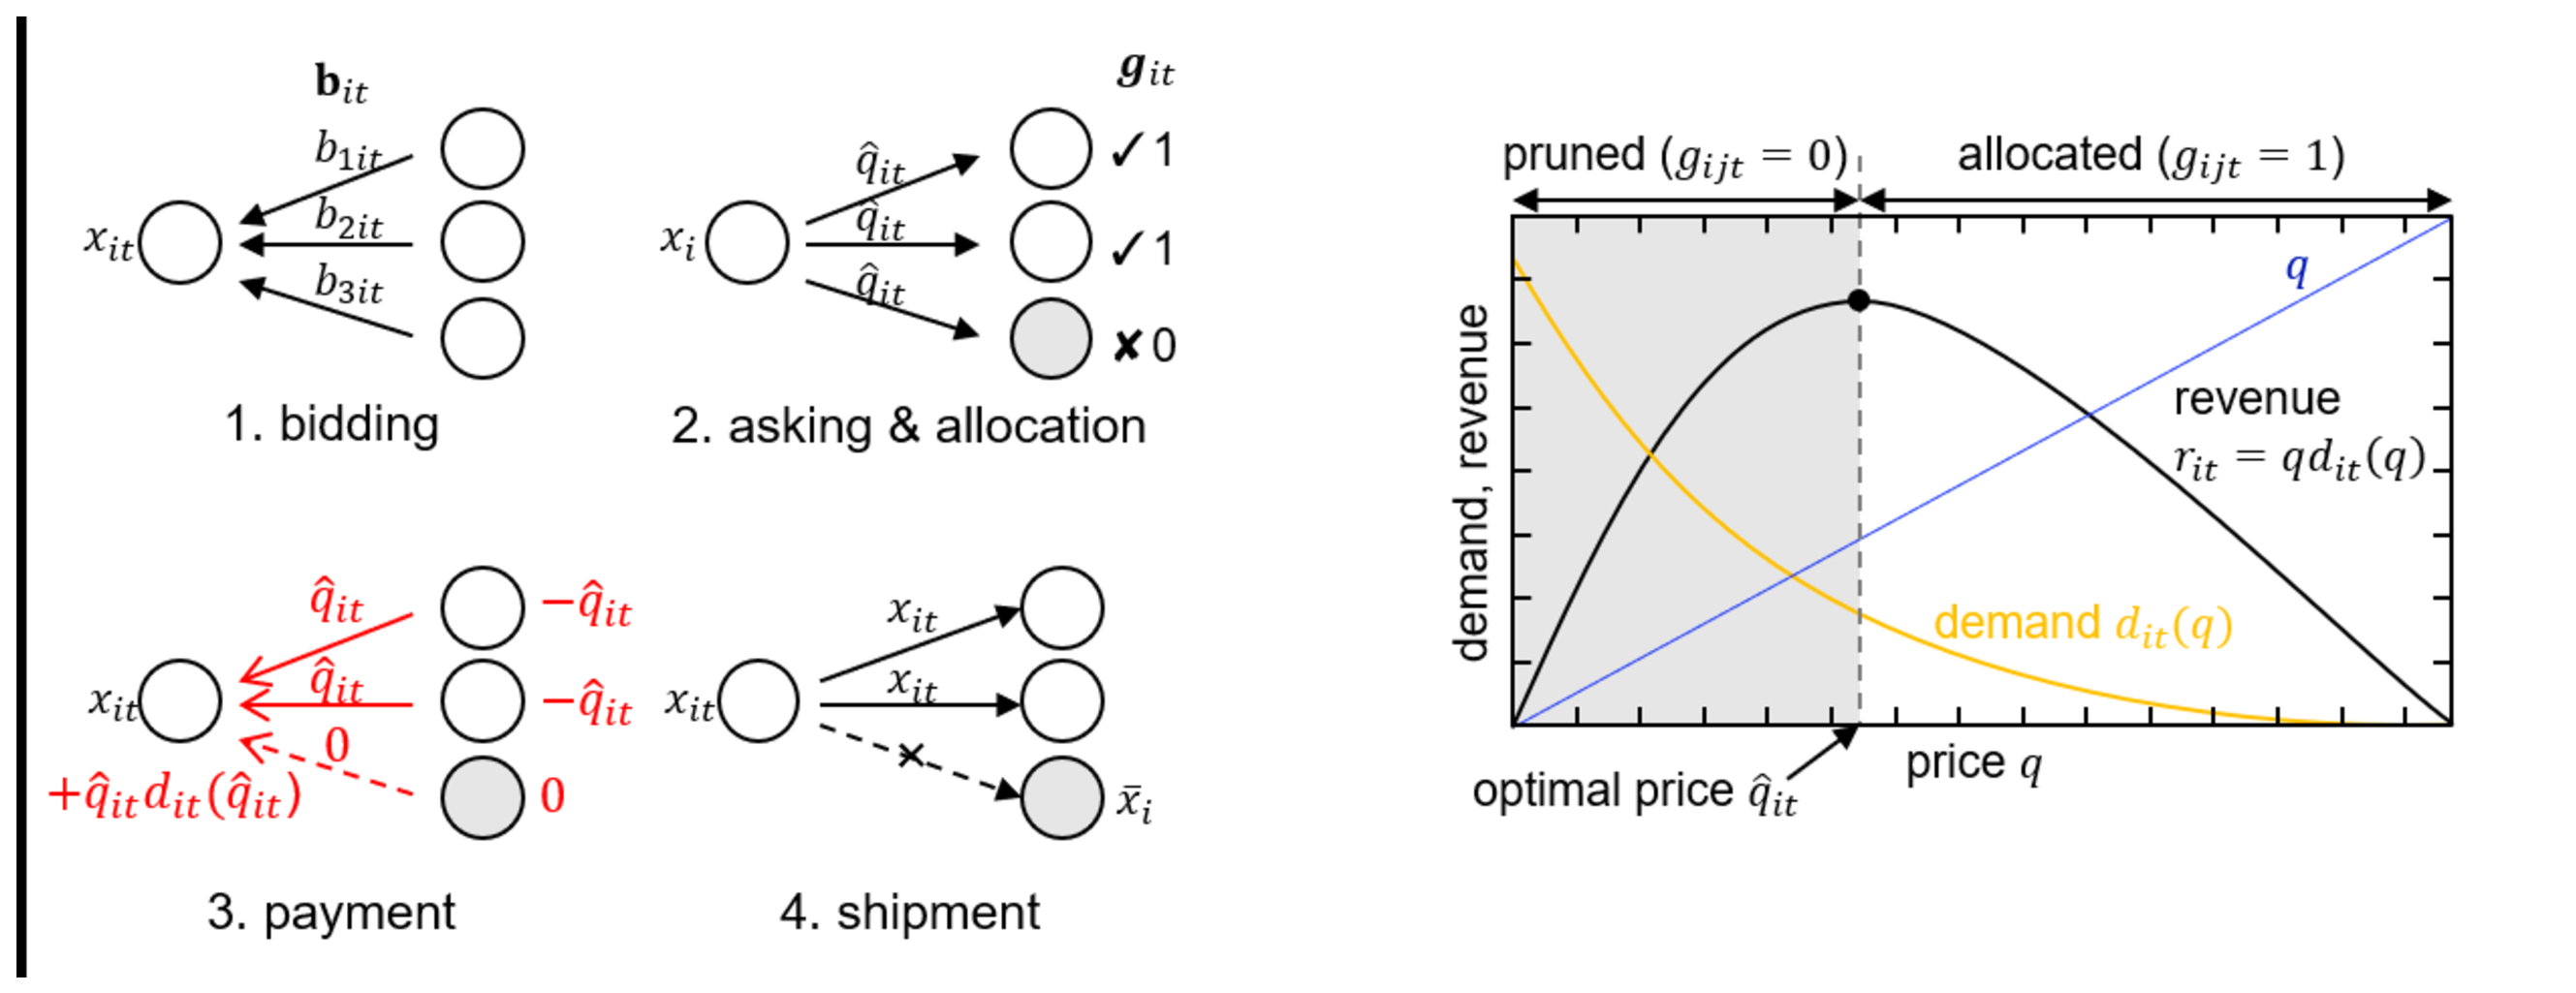
\includegraphics[width=\linewidth]{img/double.eps}
\caption{
\textbf{Left}: The process of trade in an envy-free auction.
\textbf{Right}: A price determination curve for a unit. Revenue of a unit is a product of monotonically decreasing demand and price. The price maximizing the revenue is the optimal price.
}
\label{fig:double}
\end{figure*}


Therefore, the optimization problem is presented below.
\begin{flalign}
	\max_{\vect{b}, q} \Expect{\hat{\vect{q}}_t}{ V_i^{\pi_i}(s_{it}) } = 
		\max_q q d_{it}(q) - 
		\min_{\vect{b}} \Expect{\hat{\vect{q}}_t}{\vect{g}_{it}(\vect{b})^\T( \hat{\vect{q}}_t - \gamma \vect{o}_{i,t+1}  )} + \const.
\end{flalign}
Note that $\vect{g}_{it} = H(\vect{b} - \vect{q}_t)$.
We take the expectation $\Expect{\hat{\vect{q}}_t}{\cdot}$ 
because the asked price $\hat{\vect{q}}_t$ is unknown for $v_i$, except for $\hat{q}_{it}$, and $g_{iit} = 0$.

Then, what is bidding price $b_{it}$ to maximize return?
The following theorem holds.

\begin{thm}\label{thm:optimal-bidding}
	(Truthfulness) the optimal bidding price for maximizing return is $\opt{\vect{b}}_{it} = \vect{o}_{it}$.
\end{thm}
See the Appendix for the proof.

That is, the unit should only consider its counterfactual return (!).
Consequently, in the mechanism of NaaA, the unit obeys as if performing valuation to the other units, 
and declares the value truthfully.

Then, the following corollary holds:
\begin{coro}\label{coro:optimal-bidding}
	The Nash equilibrium of an envy-free auction $(\vect{b}_{it}, q_{it})$ is $(\vect{o}_{it}, \argmax_{q} q d_{it}(q))$.
\end{coro}

The remaining problem is how to predict $\vect{o}_t$.
Although several method can be applied to this problem,
we use $Q$-learning to predict $\vect{o}_t$.
As $\vect{o}_{it}$ is difference of two $Q$s, we approximate each of $Q$.
Other RL such as SARSA and A3C can be employed.
We parametrize the state with a vector $\vect{s}_t$ 
which contains input and weight.
$\epsilon$-greedy policy with $Q$-learning typically suppose that discrete actions
So, as an action, we employ allocation $g_{ijt}$ instead of $\vect{b}_{it}$ and $q_{it}$.
The overall algorithm is shown in Algorithm 1.

\subsection{Adaptive DropConnect}
Actually, NaaA is useful not only for multi-agent RL, but also for training of the network.
Typical training algorithms of a neural network such as those of RMSProp \citep{tieleman2012lecture} and Adam \citep{kingma2014adam} are based on stochastic gradient descent (SGD).
The optimization is performed sequentially.
Therefore, the problem can be interpreted as a problem to update the state (i.e., weight) to the goal, which is minimization of the expected likelihood.

The learning can be accelerated by application of NaaA to the optimizer.
We designate the application of NaaA to SGD as {\em Adaptive DropConnect} (ADC), 
which is eventually a combination of DropConnect \citep{wan2013regularization} and Adaptive DropOut \citep{ba2013adaptive}.
We introduce ADC herein as one application of NaaA.

ADC uses NaaA for supervised optimization problem with several revisions.
First, an environment has an input state such as an image. The agent is expected to update its parameters to maximize its reward obtained from the criterion calculator.
The criterion calculator gives batch-likelihood as the reward to the agent.
The agent is a classifier which updates its weights to maximize the reward from the criterion calculator.
The weights are recorded as an internal state.
As a counterfactual return $o_{ijt}$, we used a heuristic that uses the absolute value of weight $|w_{ijt}|$, which is the
same technique as that used by Adaptive DropOut.
We use the absolute value of weights because it is the update amount for which the magnitude of error of the output of units is proportional to $|w_{ijt}|$.

The algorithm is presented as Algorithm 2.
Because the algorithm is quite simple, its implementation can be performed easily.
For that reason, it can be widely applied for most general deep learning problems such as 
image recognition, sound recognition, and even for deep reinforcement learning.

\begin{algorithm}[t]
\caption{Envy-free auction for NaaA}
\begin{algorithmic}[1]
	\FOR{ $t=1$ \TO $T$ }
		\STATE Compute a bidding price for every edge: \textbf{for} $(v_j, v_i) \in \edges$ \textbf{do} \
		$b_{ijt} \leftarrow Q^{\pi_i}( \vect{s}_{it}, \vect{e}_j) - Q^{\pi_i}( \vect{s}_{it}, \vect{0})$ 
		\STATE Compute an asking price for every node: \textbf{for} $\unit \in \units$ \textbf{do} \
		$\opt{q}_{it} \leftarrow \argmax_{q \in [0, \infty)} q d_{it}(q).$
		\FOR{$(v_i, v_j) \in \edges$}
				\STATE Compute allocation: $g_{jit} \leftarrow H(b_{jit} - \opt{q}_{it})$ 
				\STATE Compute the price the agent should pay: $\rho_{jit} \leftarrow g_{jit} \opt{q}_{it}$ 
		\ENDFOR
		\STATE Make a payment: \textbf{for} $\unit \in \units$ \textbf{do} \
		$R_{it} \leftarrow \sum_{j \in N^\mathrm{out}_i} \rho_{jit} 
				- \sum_{j \in N^\mathrm{in}_i} \rho_{ijt},$
		\STATE Make a shipment: \textbf{for} $\unit \in \units$ \textbf{do} \
		$\tilde{x}_{ijt} = g_{ijt} x_{ijt} + ( 1 - g_{ijt} ) \bar{x}_{ijt} $

		\FOR{$\unit \in \units$} 
			\STATE Observe external state $\vect{s}_{it}^{\mathrm ex}$
			\STATE $\vect{s}_{it} \leftarrow (\vect{s}_{it}^{\mathrm ex}, \vect{\tilde{x}}_{it}, \bs{\theta}_i)$
			\STATE Sample action $a_{it}^{\mathrm ex} \sim \pi_i^{\mathrm ex}(\vect{s}_{it})$
			\STATE Receive external reward $R_{it} \leftarrow R_{it} + R_{it}^{\mathrm ex}(a_{it}^{\mathrm ex})$
			\STATE Update $Q^{\pi_i}$ under the manner of $Q$-learning by calculating the time difference (TD)-error 
		\ENDFOR
	\ENDFOR
\end{algorithmic}
\end{algorithm}

\begin{algorithm}[t]
\caption{Adaptive DropConnect}
\begin{algorithmic}[1]
	\FOR{ $t=1$ \TO $T$ }
		\STATE Compute a bidding price for every edge: \textbf{for} $(v_j, v_i) \in \edges$ \textbf{do} \
		$b_{ijt} \leftarrow |w_{ijt}|$ 
		\STATE Compute an asking price for every node: \textbf{for} $\unit \in \units$ \textbf{do} \
		$\opt{q}_{it} \leftarrow \argmax_{q \in [0, \infty)} q d_{it}(q).$
		\FOR{$(v_i, v_j) \in \edges$}
				%\STATE Sample $u$ from a Bernoulli distribution: $u \sim \mathrm{Bernoulli}(\varepsilon)$
				%\STATE Sample $m$ from a Bernoulli distribution: $m \sim \mathrm{Bernoulli}(1/2)$
				\STATE Compute allocation: $g_{jit} \leftarrow H(b_{jit} - \opt{q}_{it})$ 
		\ENDFOR
		\STATE Sample a switching matrix $U_t$ from a Bernoulli distribution: $U_t \sim \mathrm{Bernoulli}(\varepsilon)$
		\STATE Sample the random mask $M_t$ from a Bernoulli distribution: $M_t \sim \mathrm{Bernoulli}(1/2)$
		\STATE Generate the adaptive mask: $M_t' \leftarrow U_t \circ M_t + (1 - U_t) \circ G_{ijt}$ 
		\STATE Compute $\vect{h}_t$ for making a shipment:
			$\vect{h}_t \leftarrow (M_t' \circ W_t) \vect{x}_t + \vect{b}_t$
		\STATE Update $W_t$ and $\vect{b}_t$ by backpropagation.
	\ENDFOR
\end{algorithmic}
\end{algorithm}


%========================================================================
% 【論旨】
% - Q-learning と \epsilon-greedy 方策による強化学習で最適化をする
%	 - 状態を入力と重みを用いてパラメトライズする
%	 - 行動として allocation \g を用いる
%	 - 報酬は profit: revenue と cost の差
%    - つまり、NaaA では結果的に全体としてパフォーマンスが向上するようコネクションを最適化する
% 	 - これはランダムにエッジを落とす dropconnect の拡張であり、より精度向上ができると考えられる。
% - NaaA に基づくネットワーク最適化を adaptive dropconnect と名付ける
%	 - 類似の事例として、過去に提案されている adaptive dropout はこれをより一般化した話
%	 - $\epsilon=0$ の場合には dropconnect と完全に等しくなる
% - Adaptive dropconnect は、強化学習以外にも応用可能
% 	 - 強化学習以外の場合は、報酬として正解に基づく 0/1 の情報を用いて、$gamma = 0$ とする。
% 	 - 実装上は層を入れ替えるだけなので簡単
% - アルゴリズム
%========================================================================

%$\vect{o}_t$ のみ用いた greedy な方策を用いると、
%方策として、$\epsilon$-greedy を用いた
%We use $\epslion-greedy$
%We show that pre $Q$ lead us t
%我々は $\epslion-greedy$ における探索は dropconnect であるため、
%adaptive dropconnect に等しいことを示す。
%
%$\epsilon$
%
%次に、adaptive dropconnect について述べる。
%
